\clearpage
% ==================== 系统运行效果展示 ====================
\section{系统运行效果展示}

为增强课程设计报告的可读性和验收展示效果，本节从\verb|docs/report/figure|目录中选取边端识别、事件管理、智能体分析、知识库管理和报告导出等代表性截图，展示系统从边端实时感知到云端复核分析、再到管理端处置与报告输出的完整运行闭环。

\subsection{边端实时识别效果}

边端工作台是系统实时运行的主要入口，能够展示摄像头画面、人体检测框、关键点骨架、当前姿态、推理状态和实时事件。图\ref{fig:edge-detection-main}展示了YOLO-Pose在边端完成目标检测与人体关键点叠加后的效果，能够直观体现端侧感知和边缘推理能力。

\begin{figure}[H]
\centering
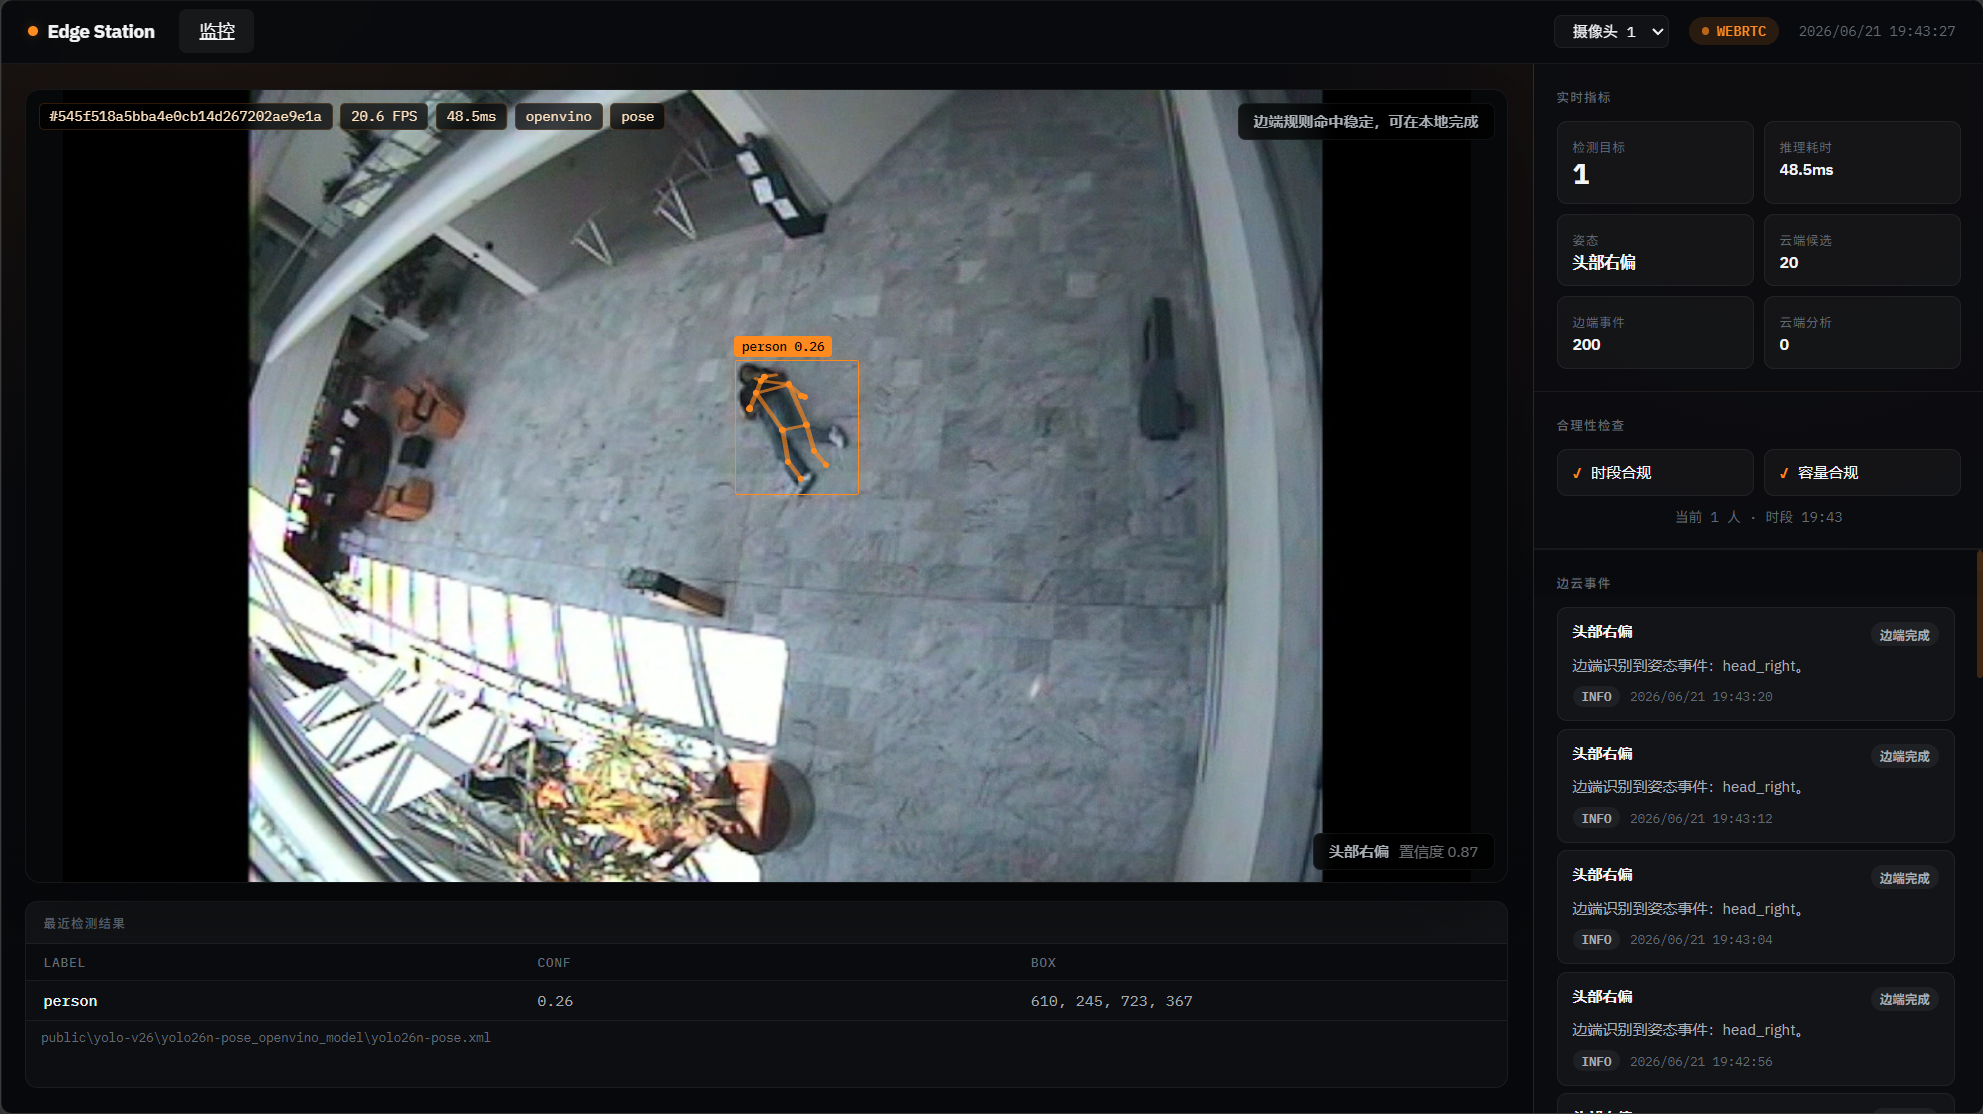
\includegraphics[width=0.94\textwidth]{figure/识别1.png}
\caption{边端实时识别与骨架叠加效果}
\label{fig:edge-detection-main}
\end{figure}

图\ref{fig:edge-detection-pose}进一步展示了姿态识别、检测结果和运行状态在前端界面中的联合呈现方式。该类界面适合课程验收时演示“摄像头采集—模型推理—姿态分析—前端可视化”的实时链路。

\begin{figure}[H]
\centering
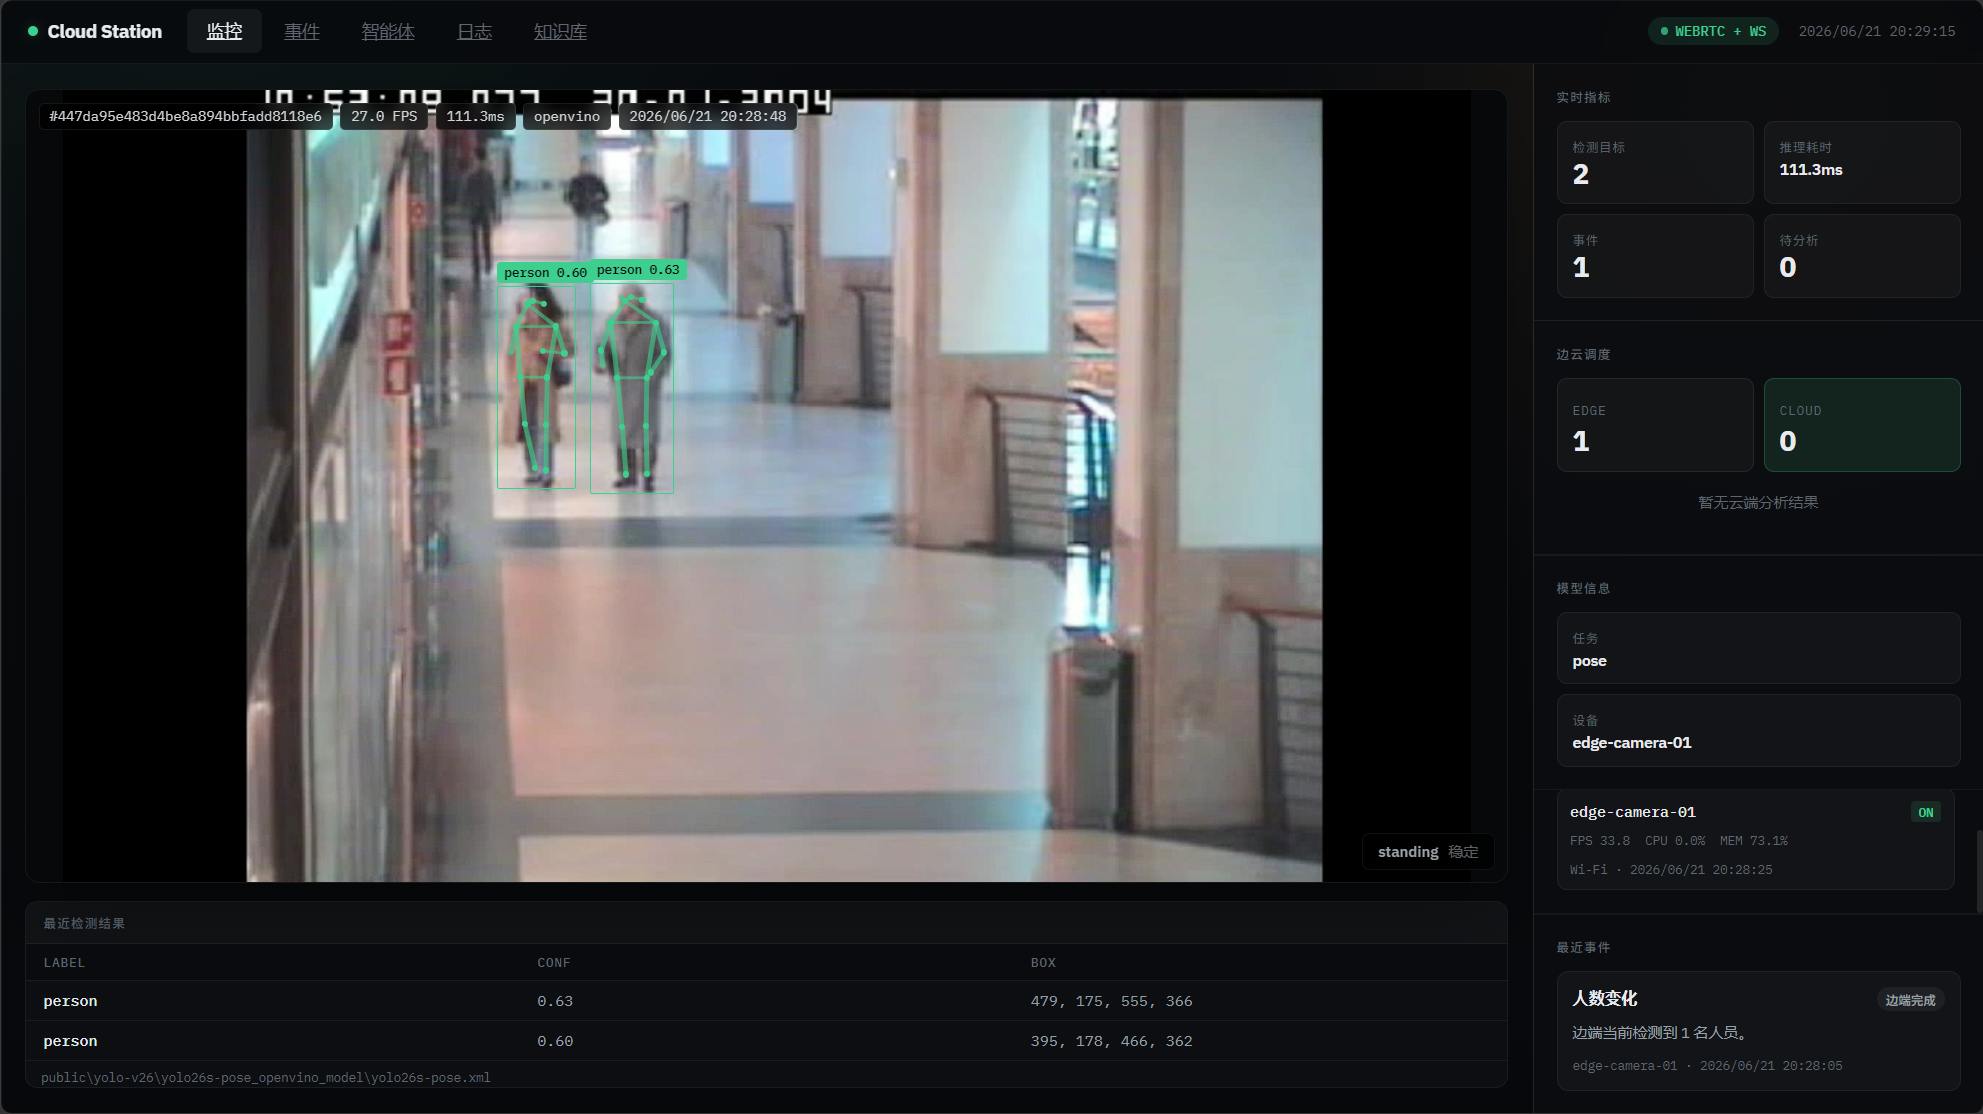
\includegraphics[width=0.94\textwidth]{figure/识别2.png}
\caption{边端姿态识别与实时状态展示}
\label{fig:edge-detection-pose}
\end{figure}

\subsection{事件管理与智能体分析}

云端控制台用于承接边端上报事件，并提供事件检索、状态管理和智能体复核能力。图\ref{fig:event-console}展示了事件列表与统计信息，体现了系统对边端事件的集中管理能力。

\begin{figure}[H]
\centering
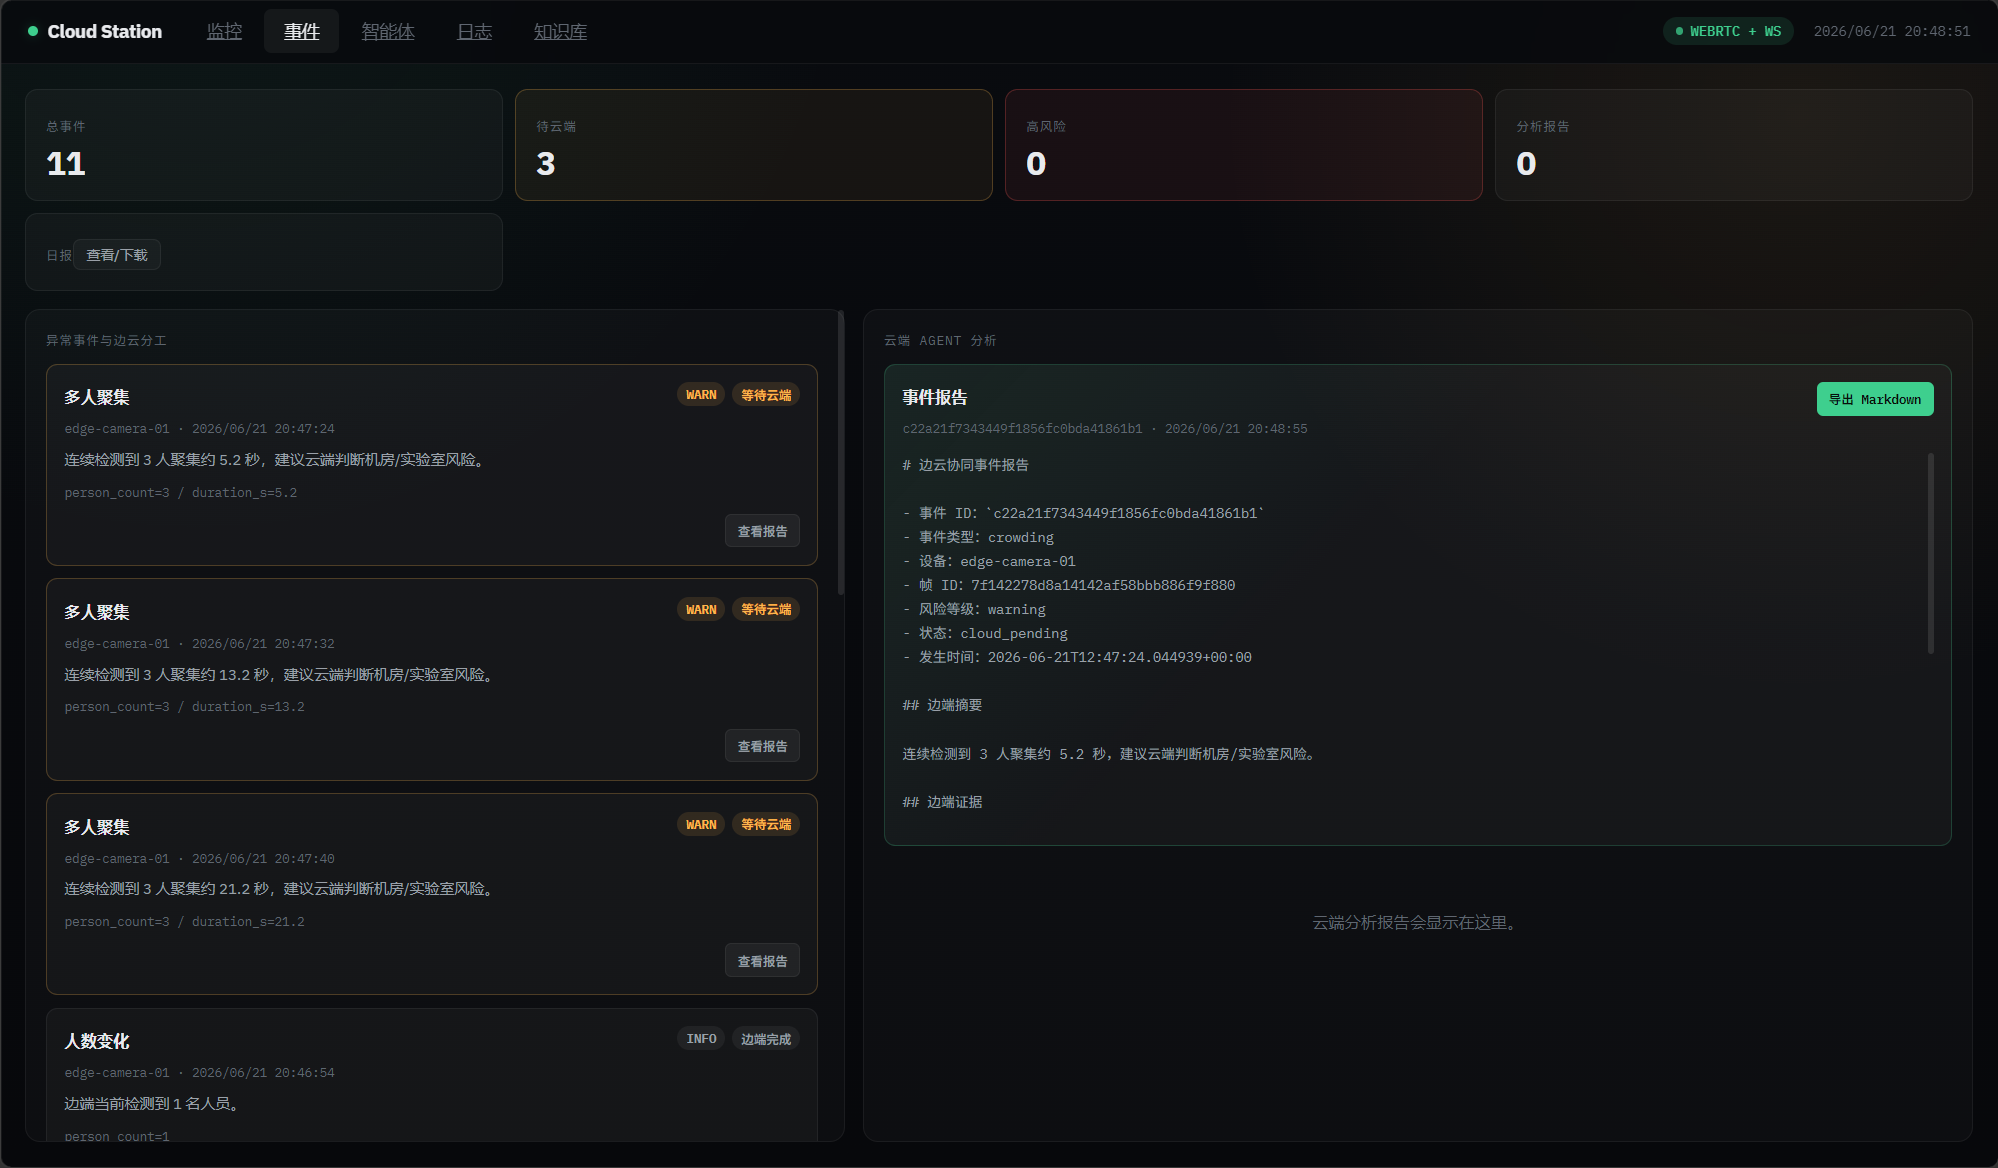
\includegraphics[width=0.94\textwidth]{figure/事件1.png}
\caption{云端事件管理与统计界面}
\label{fig:event-console}
\end{figure}

在事件复核和自然语言问答阶段，云端智能体可以结合历史事件、知识库和工具调用结果生成分析结论。图\ref{fig:agent-chat}展示了智能体交互界面，体现了系统在云端复杂分析层面的扩展能力。

\begin{figure}[H]
\centering
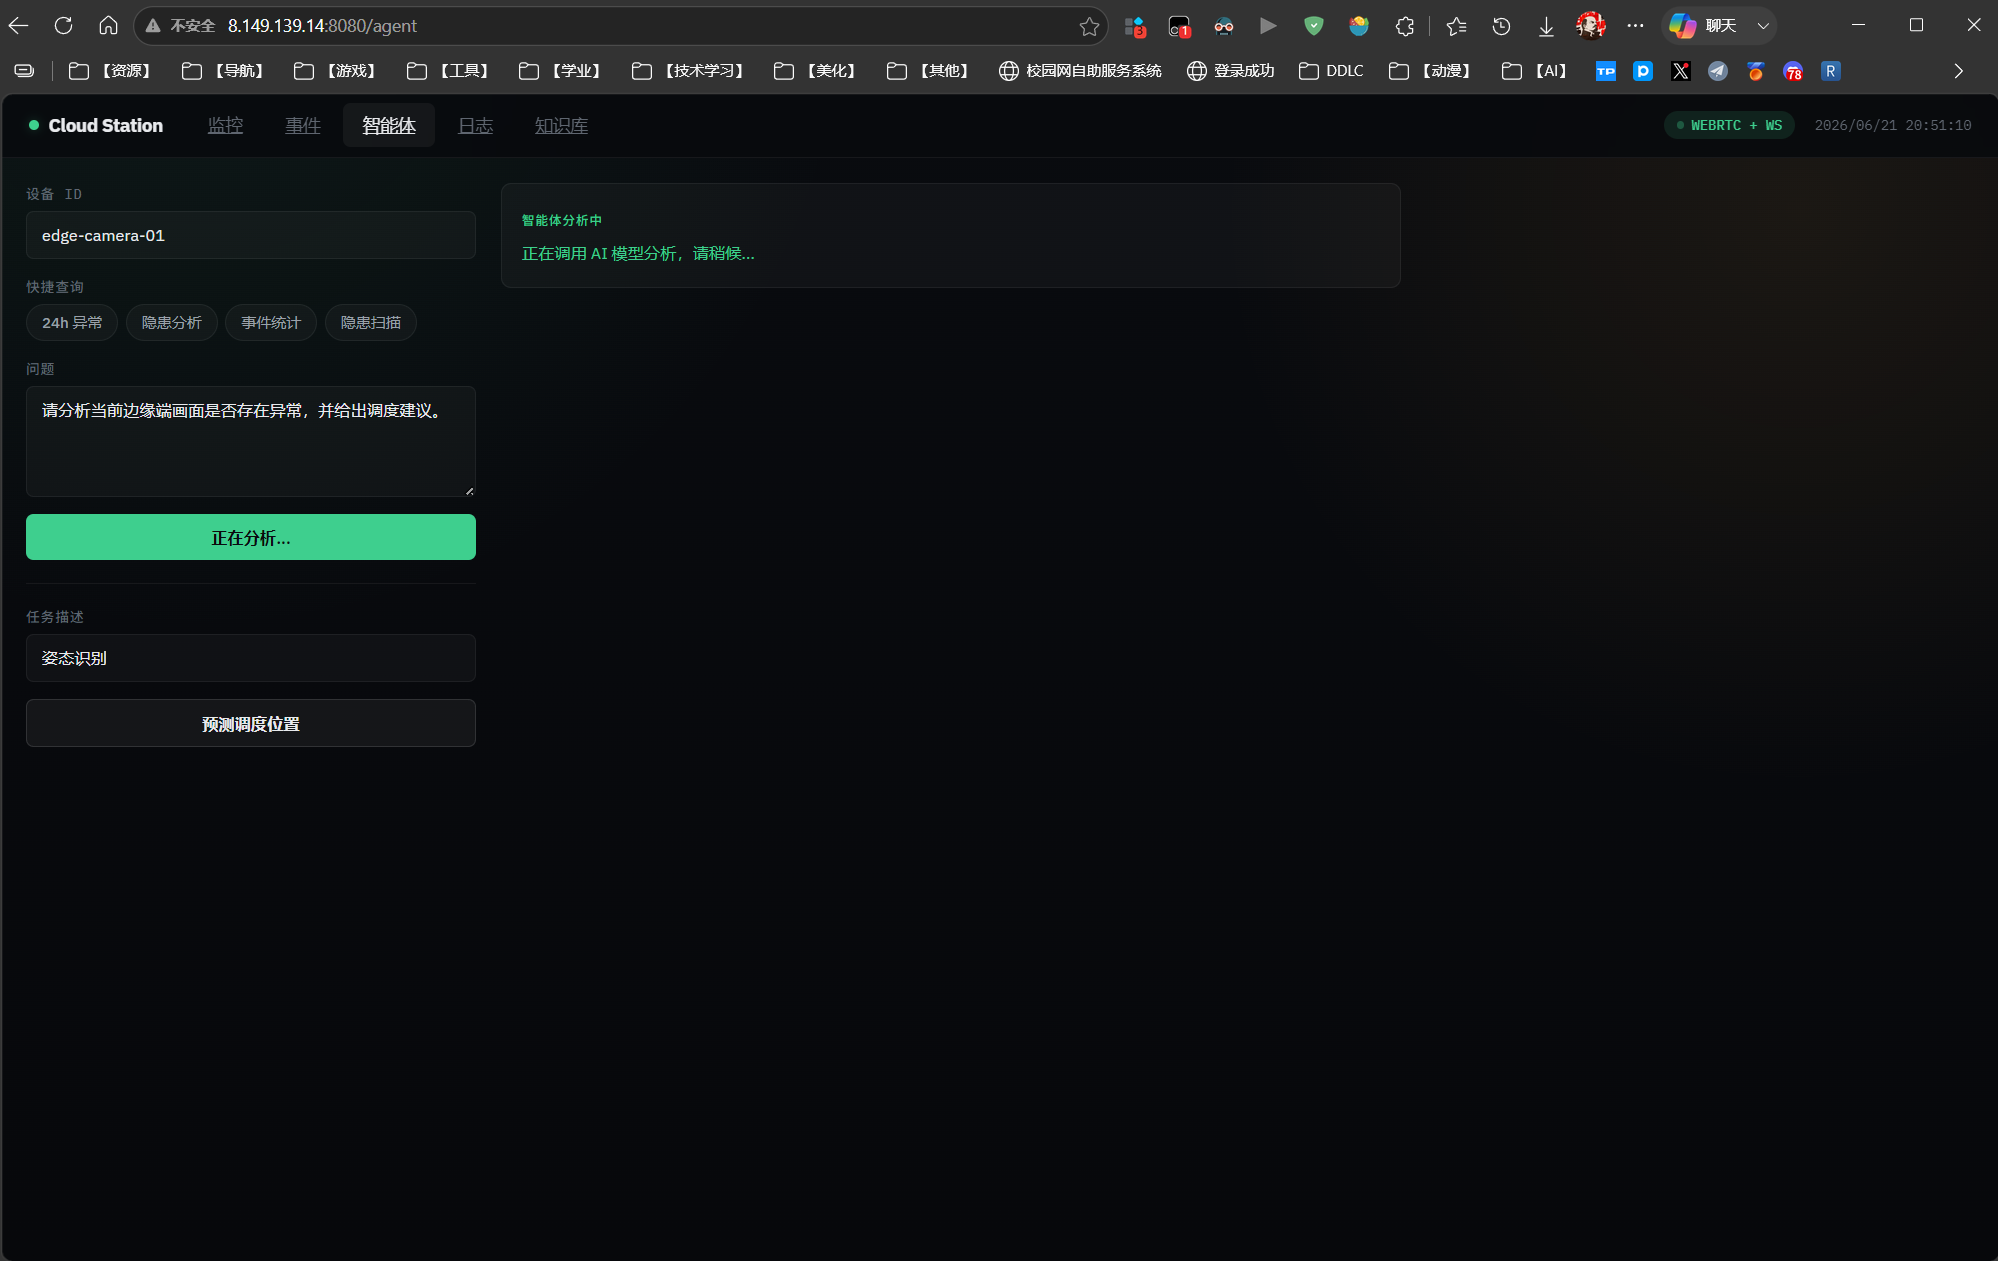
\includegraphics[width=0.94\textwidth]{figure/智能体1.png}
\caption{云端智能体问答与分析界面}
\label{fig:agent-chat}
\end{figure}

图\ref{fig:agent-report}展示了智能体分析结果生成报告后的呈现效果，用于说明系统不仅能完成实时监测，还能将事件原因、风险等级和处置建议整理为可归档材料。

\begin{figure}[H]
\centering
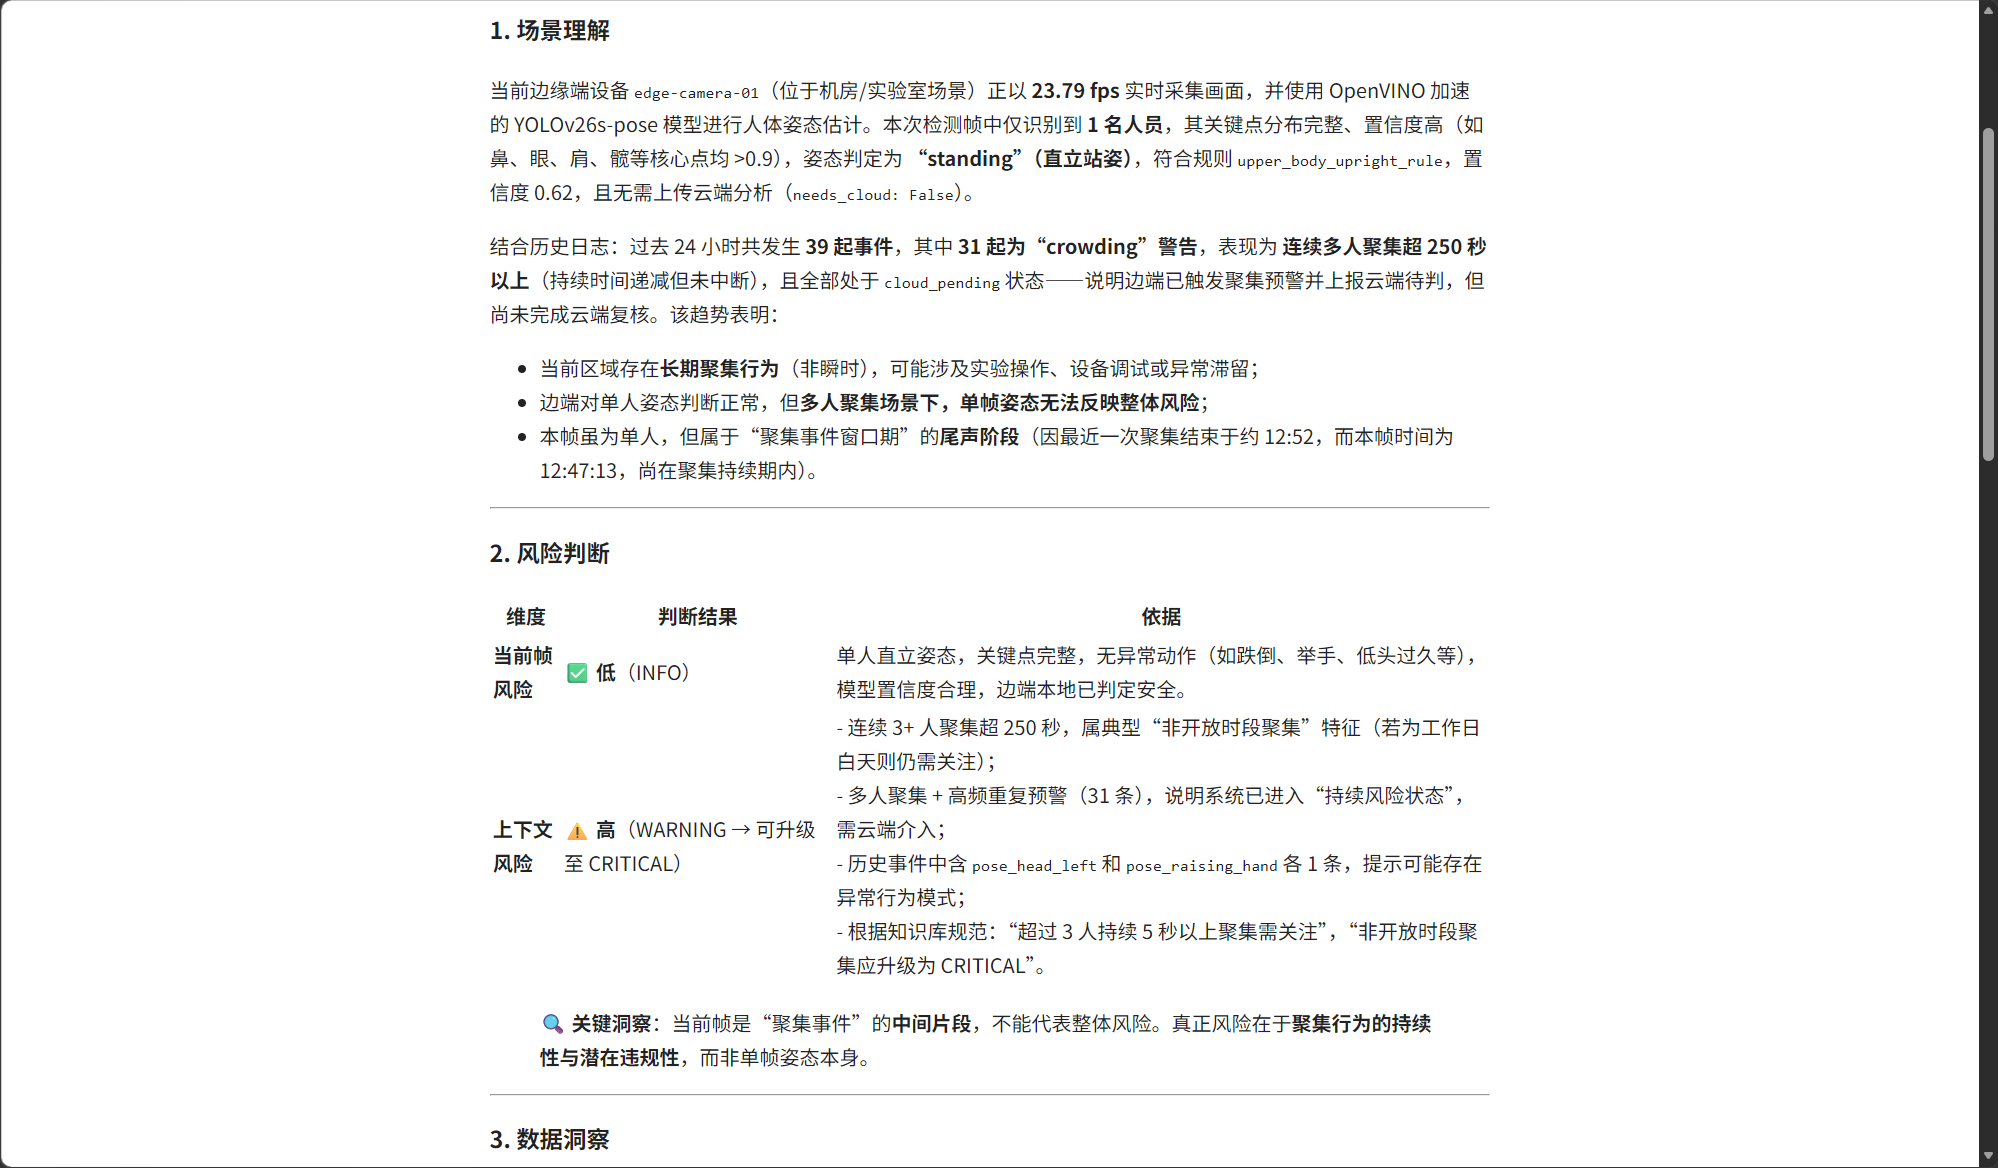
\includegraphics[width=0.94\textwidth]{figure/智能体报告2.png}
\caption{智能体检测分析报告展示}
\label{fig:agent-report}
\end{figure}

\subsection{知识库管理与日报输出}

知识库模块为智能体分析提供本地安全规范和场景说明。图\ref{fig:knowledge-base}展示了知识库文件管理与编辑界面，体现了系统对RAG资料维护的支持能力。

\begin{figure}[H]
\centering
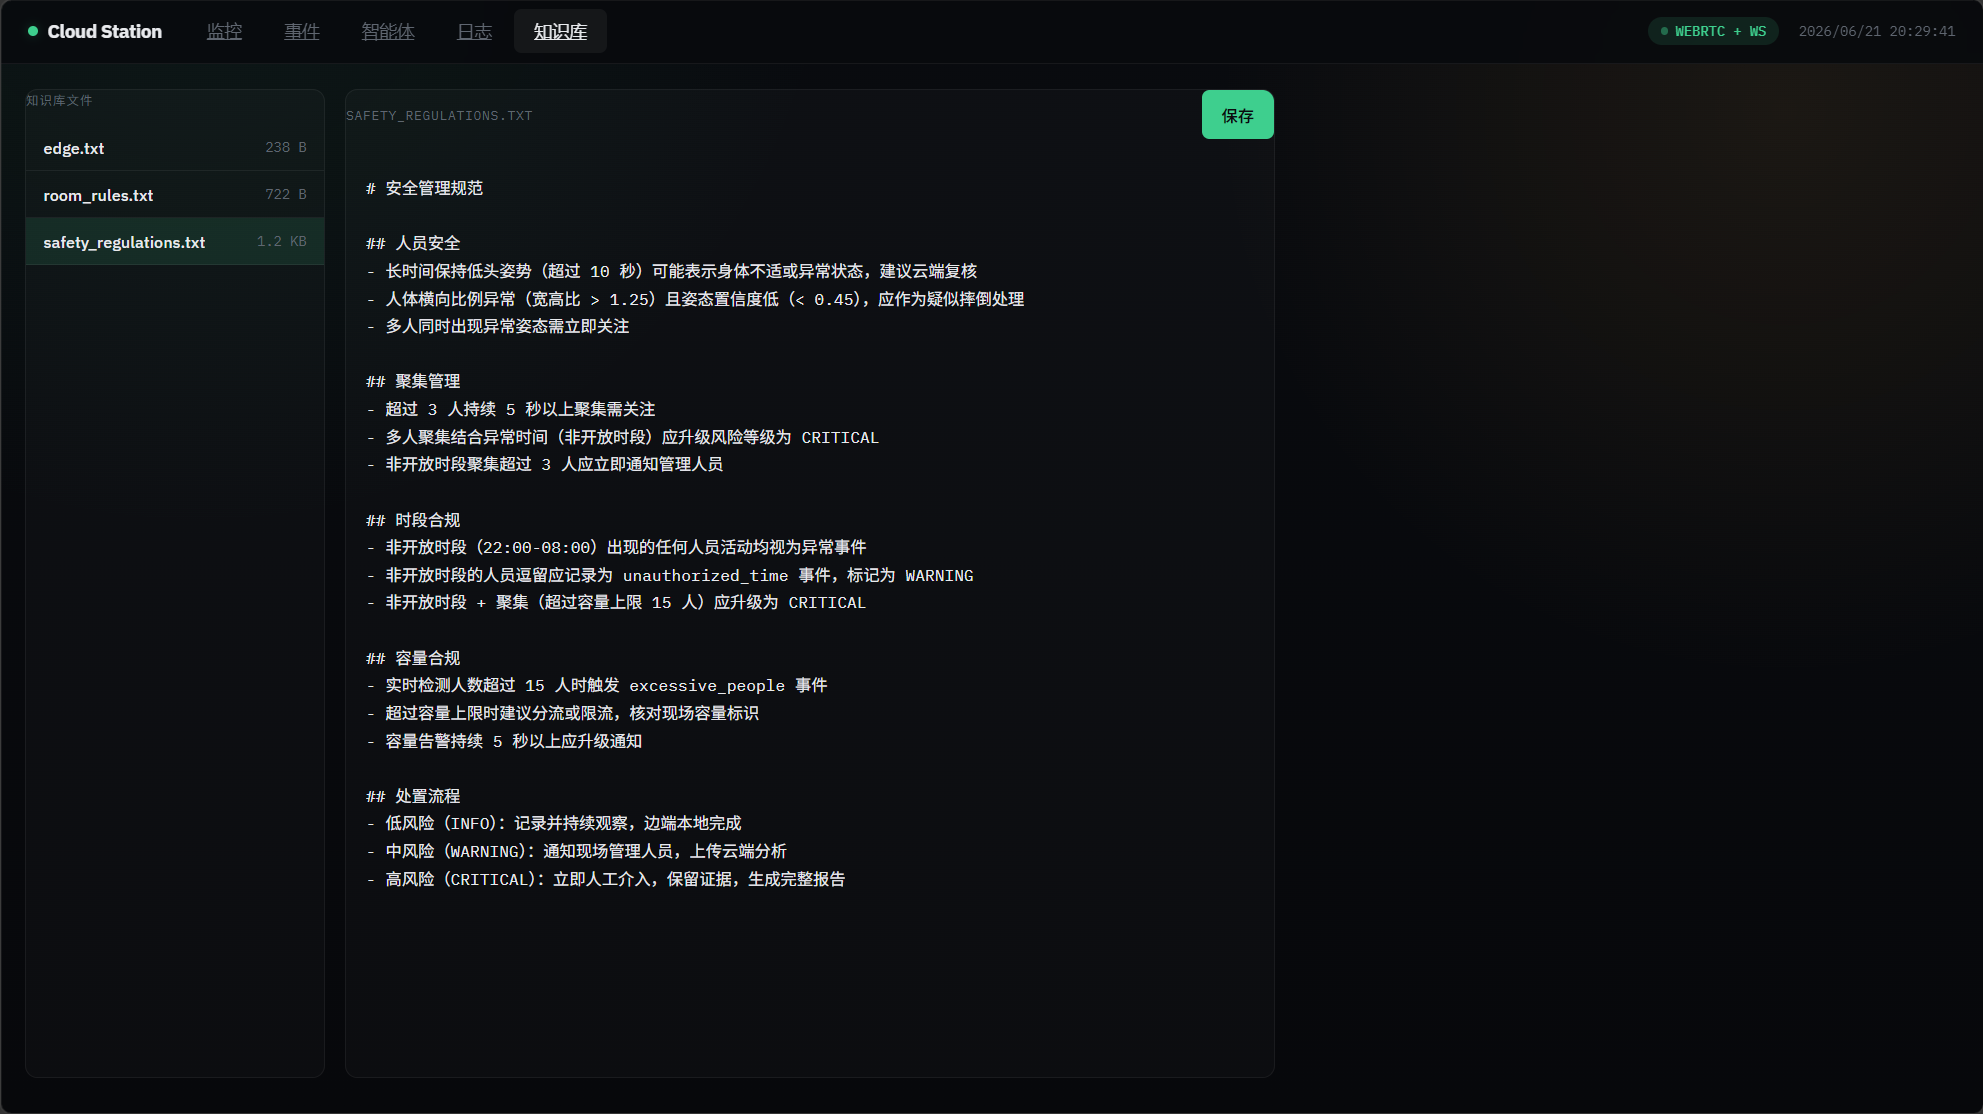
\includegraphics[width=0.94\textwidth]{figure/知识库1.png}
\caption{知识库文件管理与编辑界面}
\label{fig:knowledge-base}
\end{figure}

日报模块面向管理人员提供按日汇总的事件统计、风险概览和处置建议。图\ref{fig:daily-report}展示了日报输出界面，适合用于验收时说明系统的报告生成和后续归档能力。

\begin{figure}[H]
\centering
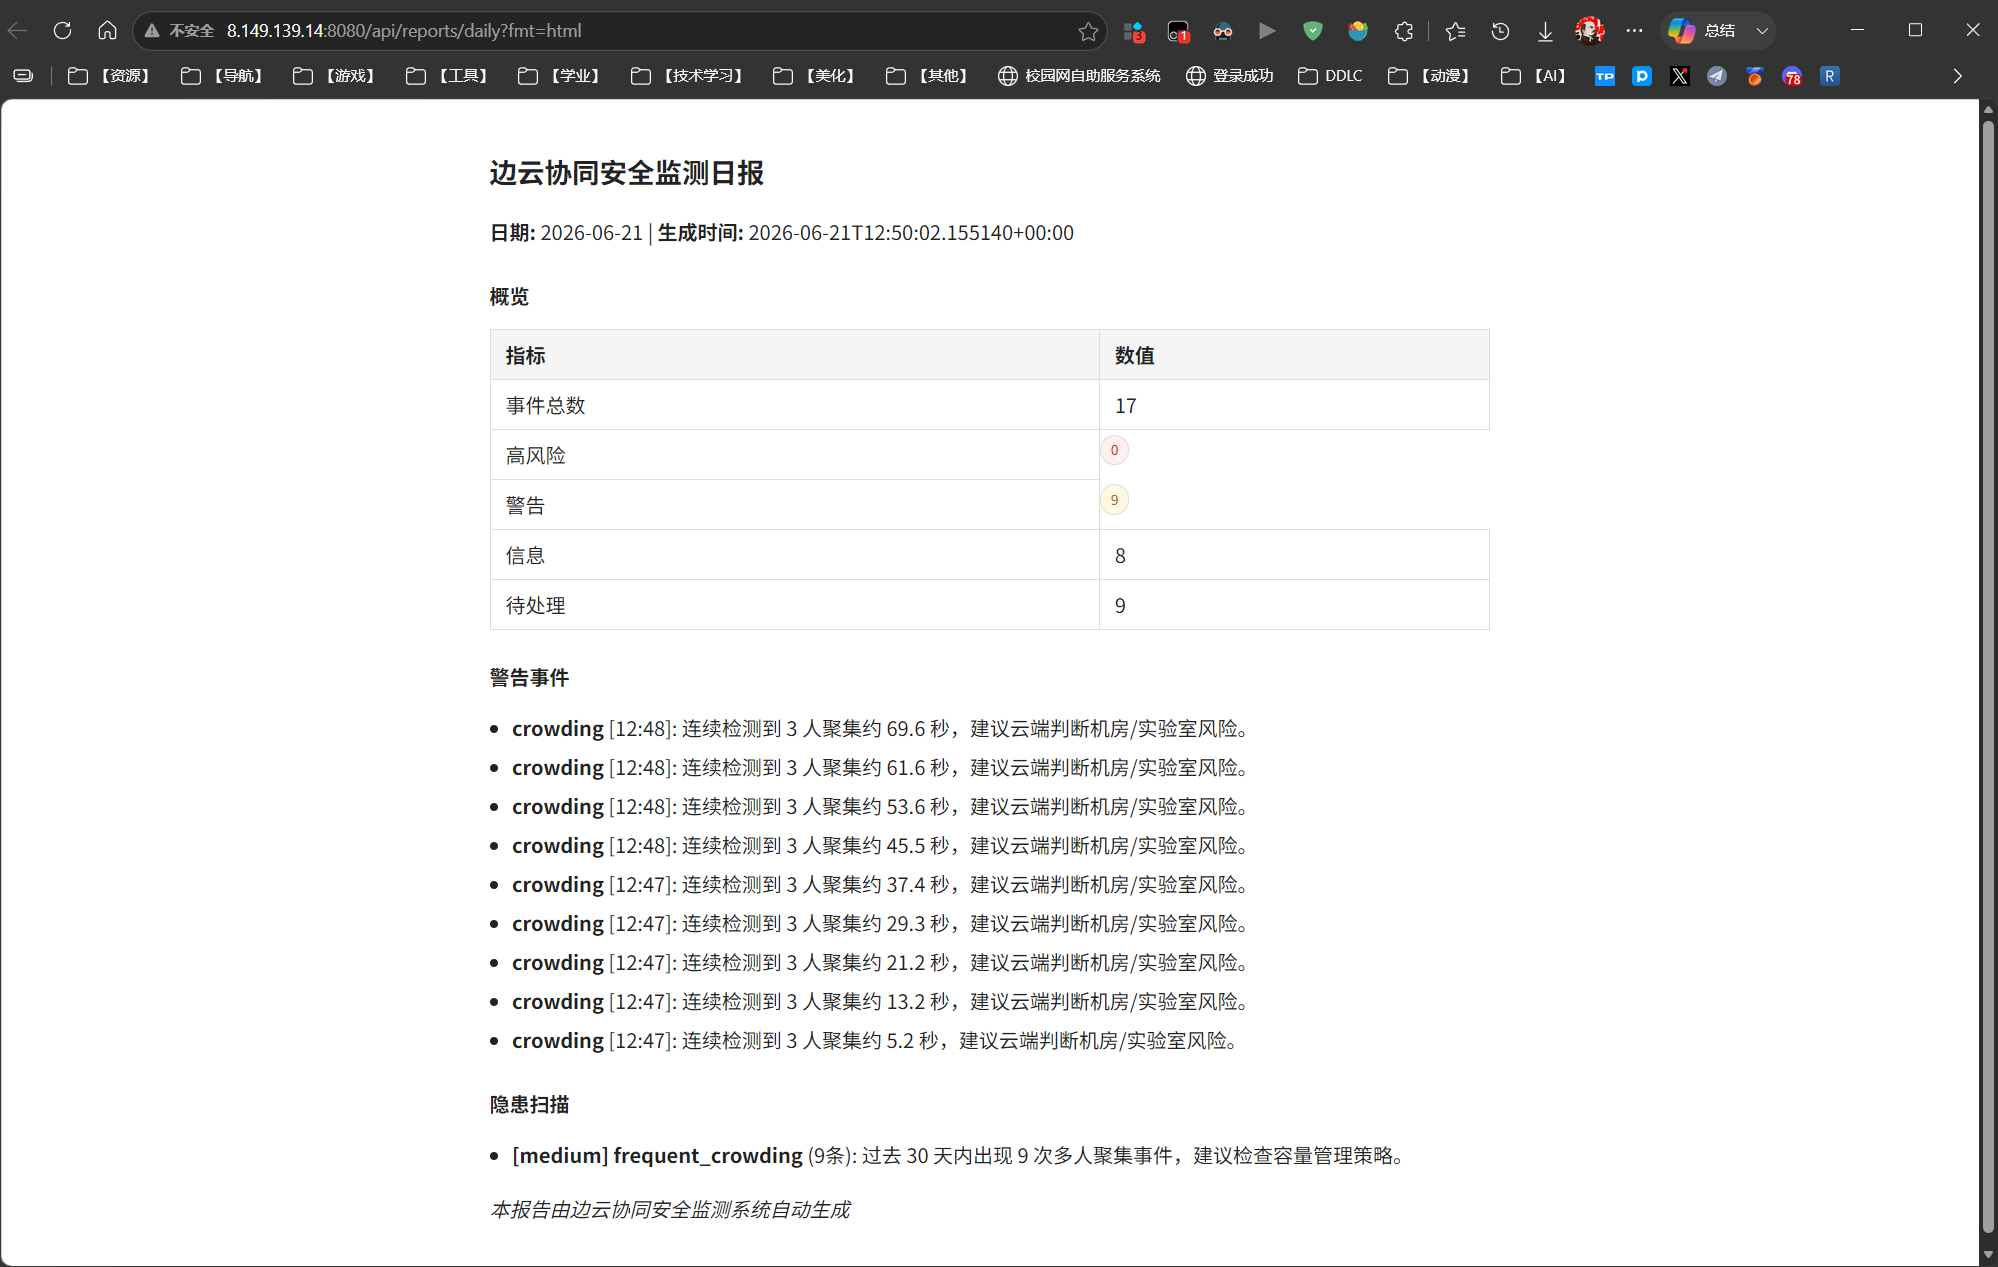
\includegraphics[width=0.94\textwidth]{figure/日报报告1.png}
\caption{日报报告展示与导出界面}
\label{fig:daily-report}
\end{figure}
